\secput{intro}{Introduction}

The \defn{predecessor} problem is to find the largest item in a given sorted list $L$
that is not greater than a query value $q$.  The \defn{iterated predecessor query} 
problem is to find the \defn{predecessor} for a query $q$ in each of a set of $k$ static lists
$L_1 \ldots L_k$, each of size $n$.  A naive solution involves individual binary searches over all
$k$ lists, which would require $O(k \lg n)$ time in the worst-case.  However, Chazelle
and Guibas~\cite{ChazelleGu86a} showed that the lists can be 
preprocessed to support iterated predecessor queries in $O(\lg n + k)$ time, with
linear preprocessing time and linear space via their technique \defn{fractional cascading}.

In this project, we will demonstrate that the iterated predecessor query problem
can be solved using a technique called \defn{range coalescing} in $O(\lg n + k)$ time.
Range coalescing is \defn{cache-oblivious}~\cite{FrigoLePr99}, using only 
$O(\log_{B+1} n + k/B)$ memory transfers to satisfy iterated predecessor
queries.  Furthermore, range coalescing requires
only linear space and the preprocessing takes linear time and $O(nk/B)$ memory
transfers.

Broad strokes of query with sweet graphic showing how the ranges are coalesced

\begin{figure}[h]
%\begin{center}
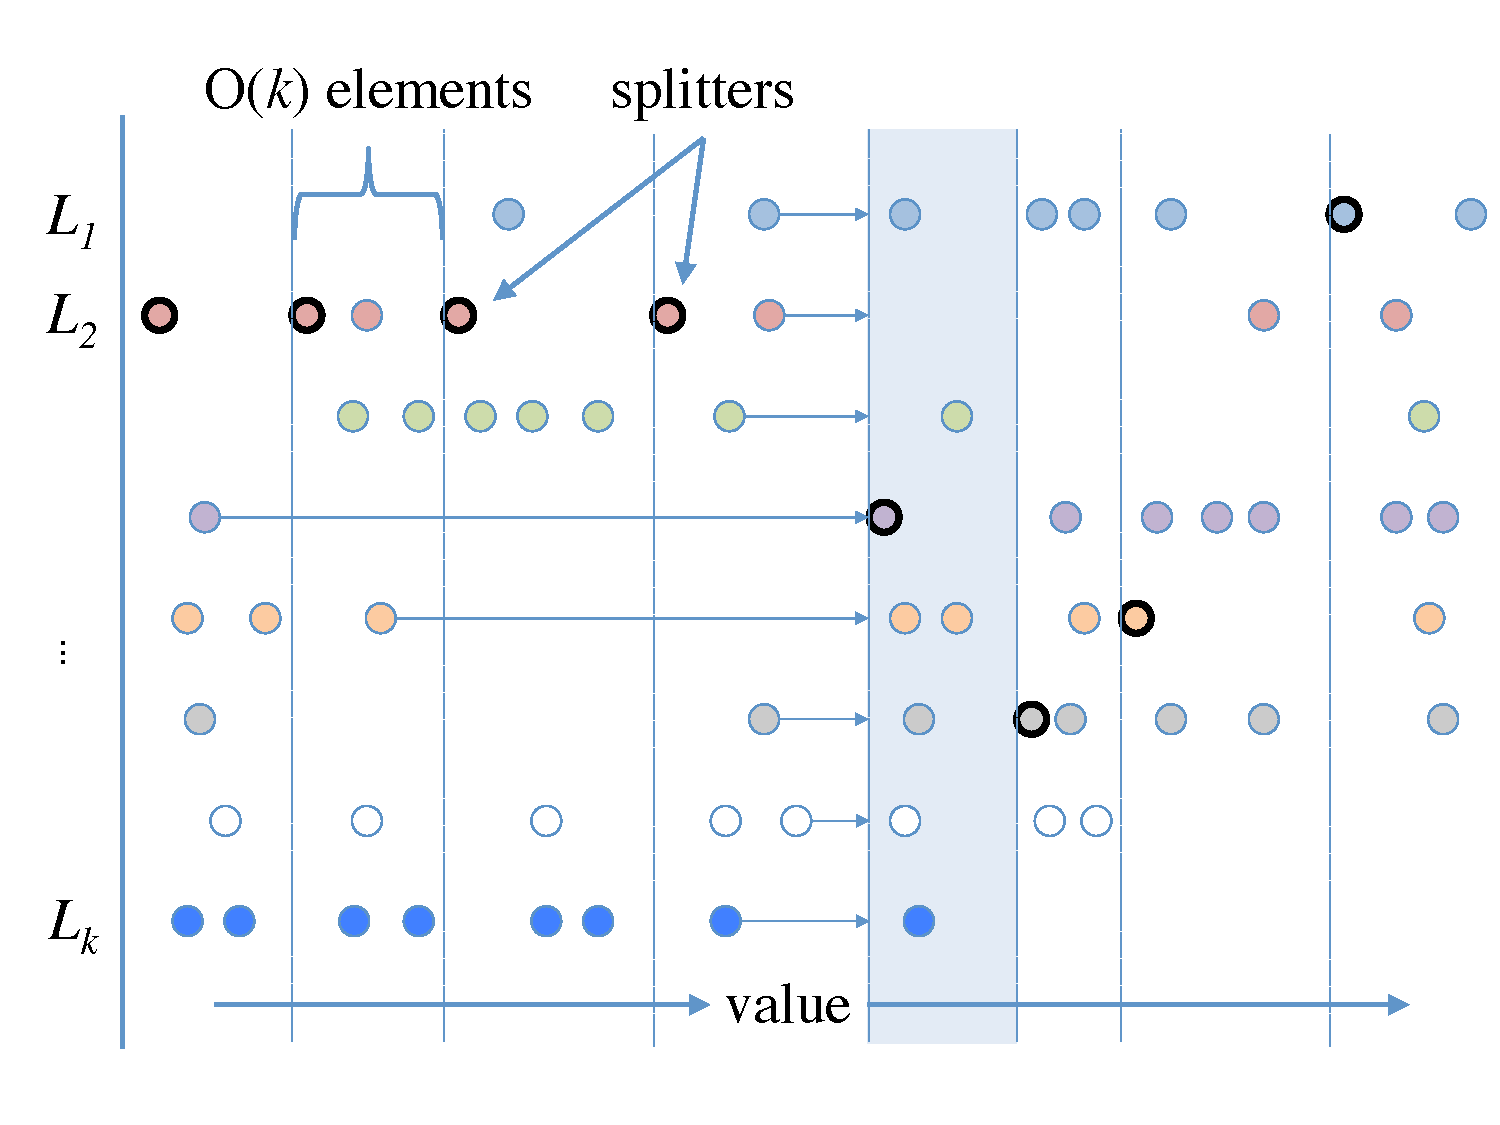
\includegraphics[scale=.3]{cache-oblivious-fractional-cascading-a.pdf}
%\end{center}
\caption{}
\label{fig:range_coalescing} 
\end{figure}

\begin{figure}[h]
%\begin{center}
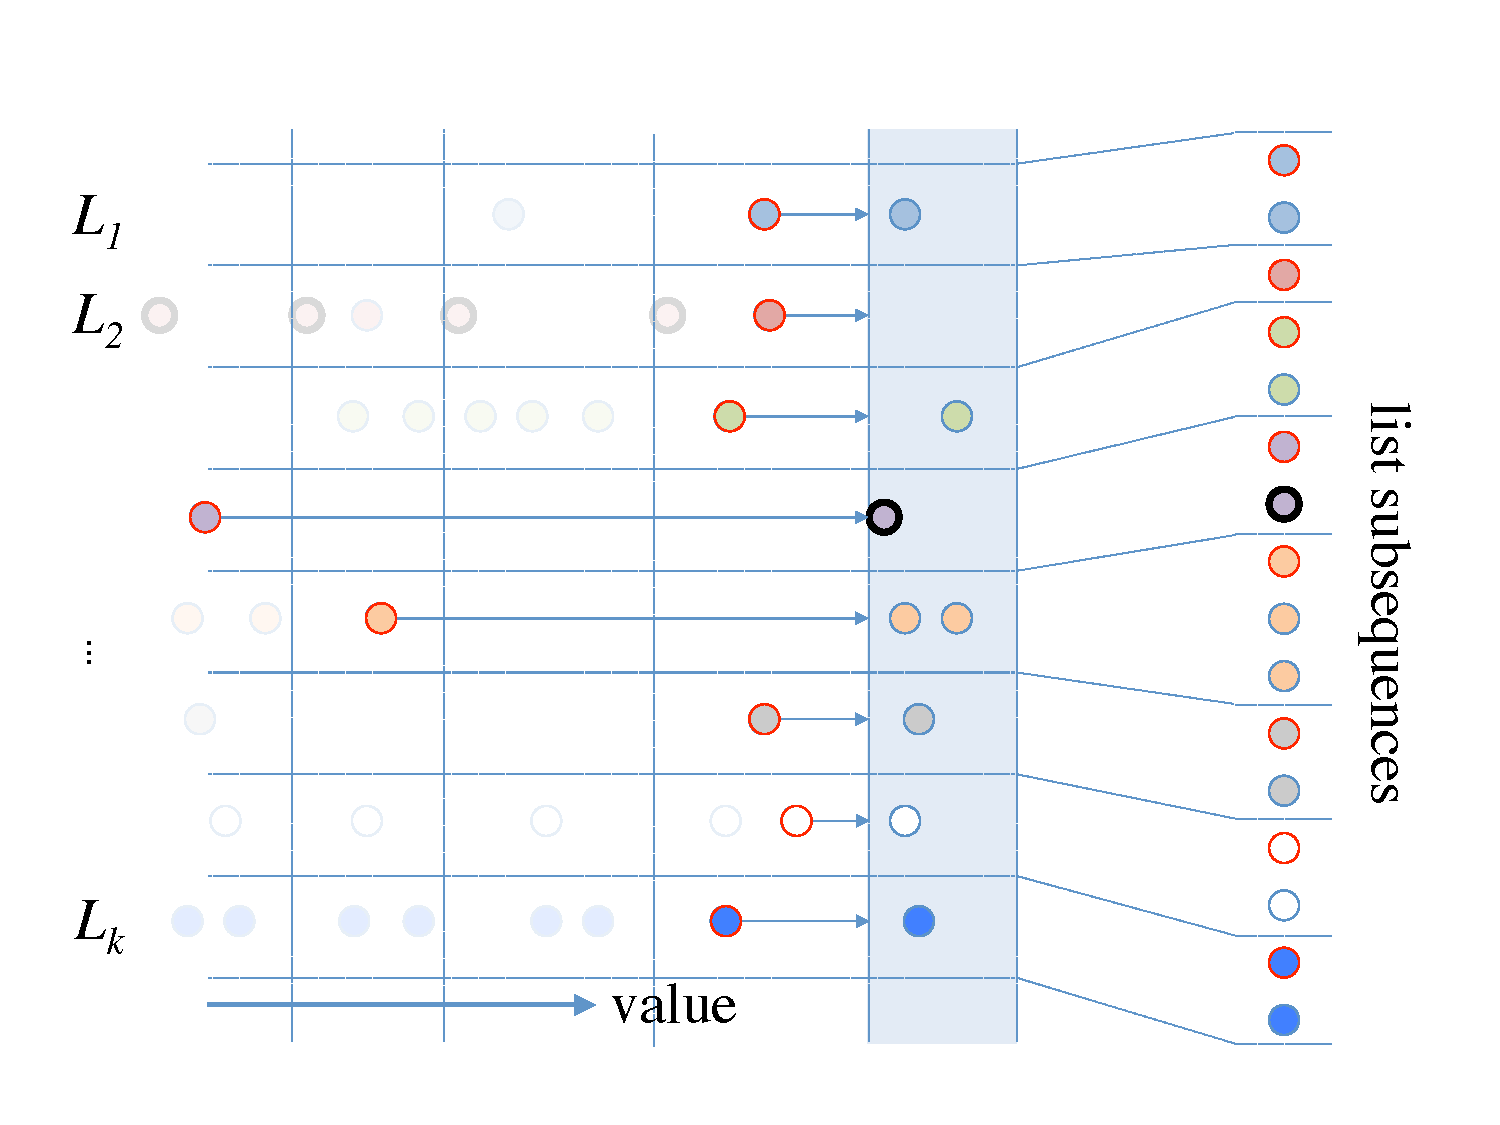
\includegraphics[scale=.33333]{cache-oblivious-fractional-cascading-c.pdf}
%\end{center}
\caption{}
\label{fig:coalesced_bin} 
\end{figure}

Terminology (define $M$, $B$ etc.)

Outline of sections
